%! TEX program = lualatex

% Use :VimtexToggleMain to compile this file alone with Vimtex
\documentclass[tikz]{standalone}

\usepackage{sty/adantikz}

\begin{document}
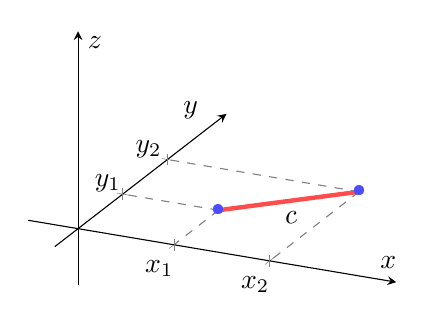
\begin{tikzpicture}[x={(8.66cm,5cm)},y={(0cm,10cm)},z={(8.66cm,-5cm)}]
\begin{axis}[
axis on top,
axis lines = center,
% Set the size of the axes
xmin = -1, xmax = 15,
ymin = -1, ymax = 15,
zmin = -1, zmax = 5,
% Show the axis labels
xlabel = $x$,
ylabel = $y$,
zlabel = $z$,
% Make the tick marks more visible
enlargelimits = 0.1,
xtick = {5, 10},
xticklabels={$x_1$,$x_2$},
ytick = {5, 10},
yticklabels={$y_1$,$y_2$},
ztick = {0},
zticklabels={$$},
% Shift the y labels to the other side
yticklabel style = {xshift={(\ticknum==0)*(-0.35cm)+(\ticknum==1)*(-0.4cm)},yshift={(0.4cm)}},
]
% Set our coordinates and draw a bar
\coordinate (p1) at (5,5,0);
\coordinate (p2) at (10,10,0);
\draw[draw=red!70,ultra thick] (p1) -- (p2) node[midway, sloped, below] {$c$};
% Draw the first point
\draw[draw=gray, dashed] (p1) -- (5,5,0);
\draw[draw=gray, dashed] (5,5,0) -- (5,0,0);
\draw[draw=gray, dashed] (5,5,0) -- (0,5,0);
\node at (p1) {\textcolor{blue!70}{\textbullet}};
% Draw the second point
\draw[draw=gray, dashed] (p2) -- (10,10,0);
\draw[draw=gray, dashed] (10,10,0) -- (10,0,0);
\draw[draw=gray, dashed] (10,10,0) -- (0,10,0);
\node at (p2) {\textcolor{blue!70}{\textbullet}};
\end{axis}
\end{tikzpicture}
\end{document}
% vim: set tw=80 ts=4 sw=4 sts=0 et ffs=unix :
